\documentclass[12pt]{acmart}

\usepackage[english]{babel}
\usepackage{amsmath, amsfonts, amsthm}
\usepackage{graphicx}
\usepackage{float}
\usepackage{multicol}

\begin{document}

\begin{titlepage}
\title{Lab 2L}
\author{6114 Chentsov Morozov}
\date{14.04.24}
\maketitle
\thispagestyle{empty}
\end{titlepage}


\tableofcontents
\newpage


\section{Web Security}

\subsection{Main Contributions}

\begin{enumerate}
    \item We define SmpSQL, an SQL fragment which is contained in $FO^2bd$;
    \item We define a a simple imperative script language SmpSL with embedded SmpSQL statements;
    \item We give a construction for weakest preconditions in $FO^2bd$ for SmpSL;
    \item We implemented the weakest precondition computation for SmpSL;
    \item We implemented a decision procedure for $FO^2bd$ The procedure is based on the decidability and NEXPTIME completeness result for $FO^2bd$ by, but we use a more involved algorithm which reduces the problem to a SAT solver and is optimized for performance.
\end{enumerate}

We evaluate our methodology on three applications: a web administrator, a simple firewall, and a conference management system. We compared our tool with $Z3$, currently the most advanced general-purpose SMT solver with (limited) support for quantifiers. In general, our tool performs better than $Z3$ in several examples for checking the validity of verification conditions of SmpSL programs. However, our tool and $Z3$ have complementary advantages: $Z3$ does well for unsatisfiable instances while our tool performs better on satisfiable instances. We performed large experiments with custom-made blown up versions of the web administrator and the firewall examples, which suggest that our tool scales well. Moreover, we tested the scalability of our approach by comparing of our underlying $FO^2$ solver with three solvers on a set of benchmarks we assembled inspired by combinatorial problems. The solvers we tested against are $Z3$, the SMT solver CVC4, and the model checker Nitpick. Our solver outperformed each of these solvers on some of the benchmarks.

\subsection{Running Example}

\subsubsection{Information}

We introduce our approach on the example of a simple web service.The example is a translation from PHP with embedded SQL commands into SmpSL of code excerpts from the Panda web-administrator. The web service provides several services implemented in dedicated functions for subscribing a user to a newsletter, deleting a newsletter, making a user an admin of a newsletter, sending emails to all subscribed users of a newsletter, etc. We illustrate our verification methodology by exposing an error in the Panda web-administrator. The verification methodology we envision in this paper consists of Table \ref{tab1} maintaining database invariants and Figure \ref{pic1} verifying a contract specification for each function of the web service.

\begin{table}[H]
\caption{Genetic algorithm parameters for simple login script}
    \begin{tabular}{|c|c|}
        \hline
        Parameters  & Values \\
        \hline
        Population size  & 30 \\
        \hline
        Survivor & 3 \\
        \hline
        Maximum Generation & 20 \\
        \hline
        Input within one individual & 2 \\
        \hline
        Type of inputs & Strings \\
        \hline
        Crossover rate (Probability) & 0.5 \\
        \hline
        Mutation rate (Probability) & 0.5 \\
        \hline
    \end{tabular}
\label{tab1}
\end{table}

\begin{figure}[H]
    \centering
    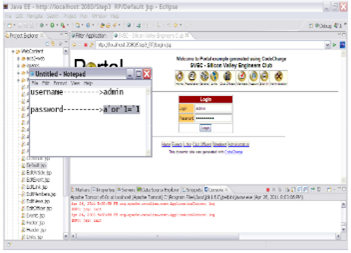
\includegraphics{Picture1.png}
    \caption{Malicious input provided to the Application}
    \label{pic1}
\end{figure}

The database contains several tables including $NS = NewsletterSubscription$ with at-butes nwl, user, subscrided and code. The database is a structure whose universe is partitioned into three sets: $domU, boolB, and codesB$. The attributes nwl and user range over the finite set $domU$  , the attribute subscribed ranges over $boolB =  (True, False)$ and the attribute code ranges over the fixed finite set $boolB$ . The superscripts in $domU, boolB, and codesB$ serve to indicate that the domain $domU$ is unbounded, while the Boolean domain and the domain of codes are bounded (i.e. of fixed finite size). When $s=true, (n,u,s,c )$ in $NS$ signifies that the user $u$ is subscribed to the newsletter $n$. The process of being (un)subscribed from/to a newsletter requires an intermediary confirmation step in which the confirm $code c$ plays a role. 

\subsubsection{Example}

Equation (\ref{1}) provides the functions subscribe, unsubscribe, and confirm translated manually into SmpSL. The comments in quotations // “. . .” originate from the PHP source code. The intended use of these functions is as follows: In order to subscribe a user $u$ to a newsletter $n$, the function subscribe is called with inputs $n$ and $u$ (for example by a web interface operated by the newsletter admin or by the user). subscribe stores the $tuple(n,u,false,new code)$ in $NS$, where new code is a confirmation code which does not occur in the database, and an email containing a confirmation URL is sent to the user $u$. Visiting the URL triggers a call to confirm with input new code, which subscribes $u$ to $n$ by replacing the $tuple(n,u,false,new code)$ of $NS$ to with $(n,u,true,nil)$. For unsubscribe the process is similar, and crucially, unsubscribe uses the same confirm function. confirm decides whether to subscribe or unsubscribe according to whether $n$ is currently subscribed to $u$. The CHOOSE command selects one row non-deterministically.\\
The database preserves the invariant

\begin{equation}
    Inv = \forall_d x,y.\forall_b s_1,s_2.\forall_c c_1,c_2 ((s_1=s_2 )\vee V_1 \neg NS(x,y,s_i,c_i )).
    \label{1}
\end{equation}

 Inv says that the pair $(n, u)$ of newsletter and user is a key of the relation $NS$. The subscripts of the quantifiers denote the domains over which the quantified variables range. In our verification methodology we add invariants as additional conjuncts to the pre- and postconditions of every function. In this way invariants strengthen the pre-conditions and can be used to prove the post-conditions of the functions. On the other hand, the post-conditions require to re-establish the validity of the invariants in Equation (\ref{2}).

\begin{equation}
    \forall_x \forall_y (a(x,y) \wedge \bigwedge_{i=1}^mF_i(x,y), B_i(x,y)) \wedge \bigwedge_{i=1}^m \forall_x \forall_y F_i(x,y).
    \label{2}
\end{equation}
 
 Equation (\ref{3}) provides pre- and post-conditions $pref and postf$ for each of the three functions $f$. The relation names $d, b, and c$ are interpreted as the sets $domU   , boolB, and codesB$, respectively. Proving correctness amounts to proving the correctness of each of the Hoare triples $\{pre.f, Inv\}  f  \{post.f, Inv\}$.

\subsection{Background}

\begin{equation}
    Precision = \frac{tp}{tp + fp'},
    \text{where}
    \label{3}
\end{equation}\\

Precision - defined in Equation 1\par
    $tp$ - the number of $true$ positives identified by the model;\par
	$fp$ - the number of $false$ positives identified by the model.

\subsection{The CNF formula}

\begin{itemize}
    \item The universe $As$ is $As$;
    \item An unary relation name $U$ is interpreted as the set $e2$;
    \item A binary relation name $R$ is interpreted in Figure \ref{pic2}.
\end{itemize}

\begin{figure}[H]
    \centering
    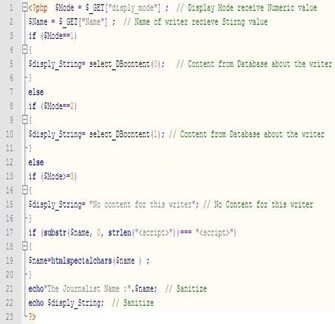
\includegraphics{Picture2.jpg}
    \caption{PHP Script of Newspaper Display Script}
    \label{pic2}
\end{figure}

\end{document}